\documentclass[journal]{IEEEtai}

\usepackage[colorlinks,urlcolor=blue,linkcolor=blue,citecolor=blue]{hyperref}

\usepackage{color,array}

\usepackage{graphicx}

\usepackage{amsmath}

\usepackage{cite}

\usepackage{algpseudocode}

\usepackage{verbatim}

\usepackage{float}

\usepackage{listings}


\definecolor{codegreen}{rgb}{0,0.6,0}
\definecolor{codegray}{rgb}{0.5,0.5,0.5}
\definecolor{codepurple}{rgb}{0.58,0,0.82}
\definecolor{backcolour}{rgb}{0.95,0.95,0.92}

\lstdefinestyle{mystyle}{
	backgroundcolor=\color{backcolour},   
	commentstyle=\color{codegreen},
	keywordstyle=\color{magenta},
	numberstyle=\tiny\color{codegray},
	stringstyle=\color{codepurple},
	basicstyle=\ttfamily\footnotesize,
	breakatwhitespace=false,         
	breaklines=true,                 
	captionpos=b,                    
	keepspaces=true,                 
	numbers=left,                    
	numbersep=5pt,                  
	showspaces=false,                
	showstringspaces=false,
	showtabs=false,                  
	tabsize=2
}

\lstset{style=mystyle}

\raggedbottom 

%% \jvol{XX}
%% \jnum{XX}
%% \paper{1234567}
%% \pubyear{2020}
%% \publisheddate{xxxx 00, 0000}
%% \currentdate{xxxx 00, 0000}
%% \doiinfo{TQE.2020.Doi Number}

\newtheorem{theorem}{Theorem}
\newtheorem{lemma}{Lemma}
\setcounter{page}{1}
%% \setcounter{secnumdepth}{0}

\begin{document}


\title{Guía preparación control 3  (Diciembre 2023)} 


\author{Ayudante: Nicolás Araya. Profesor: Rodrigo Verschae}

\markboth{Programación de software de sistemas COM2002-1 - Segundo Semestre 2023}
{Programación de software de sistemas COM2002-1 - Segundo Semestre 2023}
\maketitle

\section{\textbf{Manejo de Archivos}}

En esta sección se trata el manejo de archivos y directorios. Las formas de manejo de archivos corresponden a la creación de archivos, abrirlos, lectura, escritura y cerrar. El manejo de archivos está muy ligado a lo que sería la comunicación entre procesos pesados, pero eso se verá más adelante en la sección correspondiente.

\subsubsection{\textbf{Lo importante}} Para el control de los archivos en código es importante conocer los \textbf{File Descriptors}. Los FD corresponden a pequeños números enteros que se utilizan principalmente en código para realizar todas las operaciones existentes.

\begin{figure}[!h]
\centering
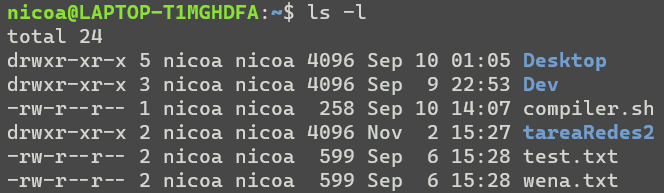
\includegraphics[width=8cm]{img/inode.png}
\caption{Implementación de ls -l, se puede apreciar en cada linea permisos del fichero, el número de enlace, nombre del propietario, nombre del grupo al que pertenece, tamaño en bytes, una marca de tiempo y nombre del fichero}
\label{fig}
\end{figure}

\begin{itemize}
\item	\textbf{ln [OPTION]... TARGET}: El comando ln corresponde al hard link que es comparable con los accesos directos. Ejemplo de uso: ln test.txt totest.txt
\item	\textbf{ls [OPTION]... [FILE]...}: ls es utilizado para ver el contenido de las carpetas. Ejemplo de uso : ls -l
\end{itemize}

\section{Operaciones}

Para las operaciones de lectura y escritura de archivos se utiliza la librería \href{https://pubs.opengroup.org/onlinepubs/7908799/xsh/unistd.h.html}{unistd.h}.

\subsection{Escritura}


\lstinputlisting[language=C]{codigos/writefunc.c}

\lstinputlisting[language=C]{codigos/writestdout.c}

En este caso, write solo retorna en la salida standar (stdout) el string.

\lstinputlisting[language=bash]{codigos/writeout.txt}

\subsection{Lectura}

\lstinputlisting[language=C]{codigos/readfunc.c}

\lstinputlisting[language=C]{codigos/read.c}

El proposito de este código es copiar los 128 bytes de la entrada estandar (stdin) a la salida estandar (stdout) .

\lstinputlisting[language=bash]{codigos/read.txt}

El método utilizado para la entrada estandar es llamado pipe, se realiza con \textbf{|} y se encarga de enviar el stdout hacia el proceso de la derecha.

\subsection{Abrir Archivos}
Open es una función atómica, lo que quiere decir que es realizada por una sola llamada a la funcion. Esto protege que varios programas intenten crear el mismo archivo al mismo tiempo.

Para abrir archivos se utiliza la librería fcntl. La sintaxis de open es la siguiente:

\lstinputlisting[language=C]{codigos/openfunc.c}

\begin{figure}[H]
\centering
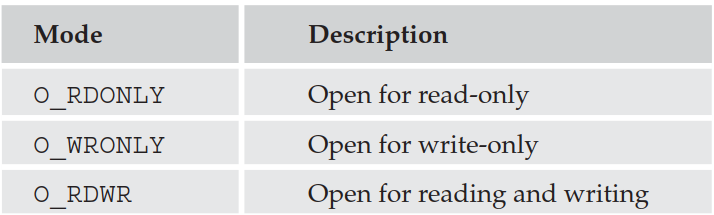
\includegraphics[width=8cm]{img/oflags.png}
\caption{Flags para especificar el tipo de operación.}
\label{fig}
\end{figure}

La forma de uso de las flags (ver Fig. 2) va de la mano con las siguientes: 

\begin{itemize}
\item	O\_APPEND: Agrega stdout de escritura al final del archivo.
\item	O\_TRUNC: Setea el tamaño del archivo a 0, ignorando el contenido.
\item	O\_CREAT: Crea el archivo tomando en consideración las flags de la Fig. 2.
\item O\_EXCL: Macro para asegurarse de que O\_CREAT haya creado el archivo. En caso de que el archivo ya exista, open falla.
\end{itemize}

Dependiendo de la situación, las flags serán true o false. La función open puede recibir varias flags mediante la operación bitwise OR ( $|$ ) y de la siguiente manera:

\begin{equation}
\text{O\_CREAT} | \text{O\_WRONLY} | \text{O\_TRUNC}
\end{equation}

Esta sería para crear un archivo de solo escritura y complementamos con O\_TRUNC para asegurarnos de ocupar toda la memoria designada. Implementado se ve:

\begin{verbatim}
open(''text.txt'', O_CREAT|O_WRONLY|O_TRUNC);
\end{verbatim}

Los permisos (ver Fig. 3) se agregan según la misma lógica:

\begin{figure}[!h]
\centering
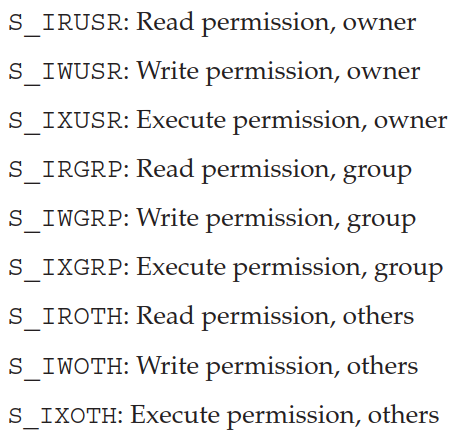
\includegraphics[width=5cm]{img/permisos.png}
\caption{Lista de permisos para open. \textbf{open(“myfile”, O\_CREAT, S\_IRUSR$|$S\_IXOTH);}}
\label{fig}
\end{figure}


\subsection{Cerrar Archivos}

\lstinputlisting[language=C]{codigos/closefunc.c}

Como se mencionó anteriormente el File Descriptor es utilizado para todas las operaciones. La función open retorna un File Descriptor que podemos utilizar posteriormente para realizar las operaciones correspondientes al archivo que hemos abierto. Por ejemplo:

\lstinputlisting[language=C]{codigos/close.c}

\lstinputlisting[language=bash]{codigos/close.txt}


\subsection{Ejercicios}

Con lo aprendido, crear un código para la copia de archivos:

\subsubsection{Paso 1}

Librerías:

\lstinputlisting[language=C]{codigos/ex1p1.c}

\subsubsection{Paso 2}

Abrir archivos de lectura y escritura:

\lstinputlisting[language=C]{codigos/ex1p2.c}

\subsubsection{Paso 3}

Lectura del archivo:

\lstinputlisting[language=C]{codigos/ex1p3.c}

\subsubsection{Paso 4}

Escritura del archivo:

\lstinputlisting[language=C]{codigos/ex1p4.c}

\subsubsection{Propuesto 1} Incrementa la cantidad de char que escribe desde el fd de lectura hacia el fd de lectura y haz que reciba el archivo desde la entrada estandar. Pista: Usa un buffer del tamaño de los char que quieres.

\subsubsection{Propuesto 2} Según la cátedra de manejo de archivos y esta guía realizar lo siguiente:

\begin{itemize}
\item \textbf{a)} Crear código para cambio de nombre, donde el nombre se recibe mediante un pipe: echo NombreArchivo $|$ ./codigo
\item \textbf{b)} Cree un link duro para un archivo ya existente y realize a) con link duro para ver que pasa.
\item \textbf{c)} ( Precaución, realizar con las medidas adecuadas. Puede tomar tiempo ) Si tiene una máquina virtual, \textbf{crear otra que no tenga nada importante} y elimine el sistema con chmod y unlink. Puede usar la obtención de inode para explorar los permisos de los archivos y encontrar el adecuado.
\end{itemize}

\section{Directorios}

A continuación se mencionarán funciones útiles para la manipulación de los directorios en un sistema Unix.

\subsection{Opendir}

\lstinputlisting[language=C]{codigos/opendir.c}

Según la dirección que se entrega abre el directorio correspondiente y retorna un puntero hacia la estructura DIR en caso de ser una llamada exitosa.

\subsection{Readdir}

\lstinputlisting[language=C]{codigos/readdir.c}

Este es llamado a través de una estructura que representará todos los atributos del directorio. Se recomienda ver la última ayudantía grabada.

\subsection{Telldir}

\lstinputlisting[language=C]{codigos/telldir.c}

Se utiliza para obtener el valor de la posición actual del directorio.

\subsection{Seekdir}

\lstinputlisting[language=C]{codigos/seekdir.c}

La función seekdir establece el puntero de entrada de directorio en el flujo de directorio dado por dirp. El valor de loc, utilizado para establecer la posición, debe haberse obtenido de una llamada previa a telldir explicada anteriormente.


\subsection{Closedir}

\lstinputlisting[language=C]{codigos/closedir.c}

\subsection{Pasos para el manejo de directorios}

\begin{itemize}
\item	Declarar puntero a directorio DIR *dp;
\item	Llamar a la estructura dirent y al atributo *entry;
\item	Asignar un directorio a dp mediante opendir u otros.
\item Realizar una lectura de los directorios mediante readdir u otras funciones del mismo fin.
\end{itemize}

\lstinputlisting[language=C]{codigos/exampledir.c}

\subsubsection{\textbf{Propuestos manejo directorios}} Realizar un programa de escaneo de directorios. Este debe entregar los subdirectorios y los archivos correspondientes. Puede guiarse de la ayudantía grabada.


\section{Procesos Pesados}

Como hemos visto a lo largo del curso, existen 2 tipos de procesos, los procesos livianos o threads y los procesos pesados.
En este caso nos enfocaremos en los procesos pesados que corresponden a un puntero a un espacio de memoria de uno o más hilos ejecutandose y que requiere de recursos para sus hilos.

\subsection{Partes de un proceso pesado}

Al momento de explorar en nuestra shell de unix utilizando por ejemplo los comandos \textbf{ps -af} o \textbf{htop} (siendo estos comandos para administrar y ver los procesos activos) podemos descubrir que cada proceso tiene códigos que lo identifican. Estos códigos son llamados PID o Process ID, es importante tener en cuenta esto al momento de trabajar con procesos pesados.

Recordando la estructura de un espacio de memoria destinado a la ejecución de procesos pesados/programas tenemos el siguiente ejemplo (ver Fig. 4):

\begin{figure}[H]
\centering
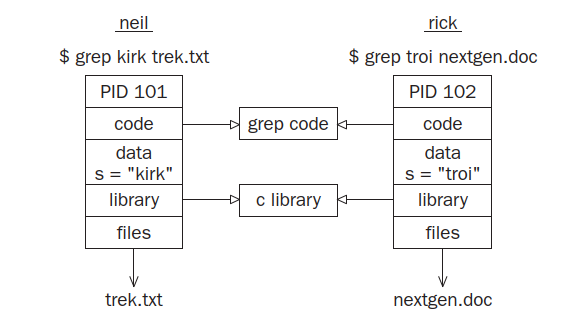
\includegraphics[width=8cm]{img/PID.png}
\caption{Corresponde a 2 procesos creados por los usuarios rick y neil.}
\label{fig}
\end{figure}

\subsection{Comenzando un nuevo proceso}

En la consola de unix, existe una forma de realizar ejecuciones de procesos a través del stdout llamado \textbf{sh -c} donde sh corresponde al comando utilizado para la ejecución de código bash y al agregar la flag -c nos permite ejecutar comandos de consola.

\lstinputlisting[language=C]{codigos/system.c}

La función system, puede hacer que se ejecute un programa dentro de otro programa creando un nuevo proceso, esto porque system realiza un sh -c en el string que se le entregue.

El siguiente código es una implementación de system:

\lstinputlisting[language=C]{codigos/system2.c}

Puede probar la función implementando más funciones que usted conozca de unix.

En general, utilizar system está lejos de ser la forma ideal de iniciar otros procesos, porque llama al programa deseado utilizando la consola. Esto es ineficaz, porque se inicia un intérprete de comandos antes de que se inicie el programa.

\subsection{Reemplazar imagen de proceso}

Las funciones \textit{exec} reemplazan el proceso actual por uno nuevo especificado por una dirección de archivo o un archivo que recibe como argumento.

\lstinputlisting[language=C]{codigos/exec.c}

Utilizando exec para inicializar el programa \textbf{ps} se puede escoger uno de los 6 exec y utilizarlos de la siguiente manera:

\lstinputlisting[language=C]{codigos/execexe.c}

Una buena práctica corresponde a utilizar el comando whereis ``comando'' para saber la ubicación del comando Unix y poder llamarlo desde exec.

\subsubsection{\textbf{Propuesto}} Implemente con cada uno de los 6 exec el comando \textbf{ls}.

\subsection{Duplicar imagen de proceso}

Para duplicar la imagen de un proceso se utiliza la función fork. Esta crea una nueva entrada en la tabla del proceso con los mismos atributos originales. Este proceso es similar al original, pues contiene los mismos atributos, pero se encuentra en otro espacio de memoria (ver Fig. 5).

\lstinputlisting[language=C]{codigos/fork.c}

\begin{figure}[h!]
\centering
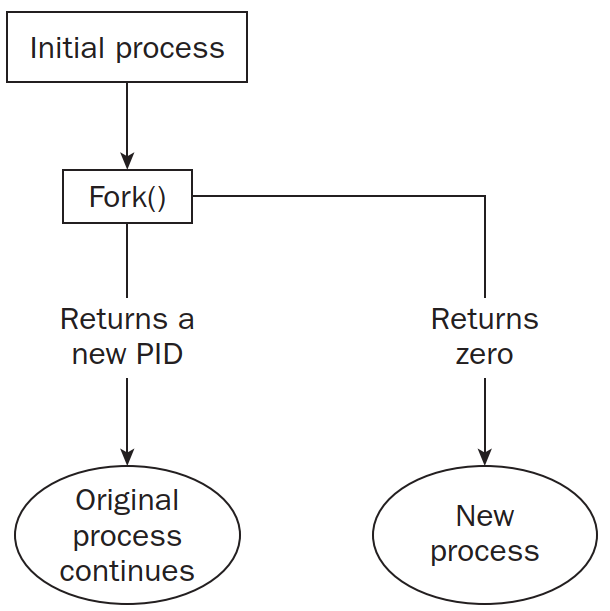
\includegraphics[width=7cm]{img/fork.png}
\caption{Corresponde a una representación del funcionamiento de la duplicación de imagen.}
\label{fig}
\end{figure}

Dependiendo del valor de retorno de la función fork existen los siguientes casos primordiales:

\begin{itemize}
\item	Caso pid\_t es -1: Si es valor de retorno es -1, es porque ocurrió un error en la creación de un nuevo proceso. Esto puede deberse a las propias limitaciones del sistema generalmente.
\item	Caso pid\_t es 0: Si es valor es 0, es porque estamos en el proceso hijo correspondiente a la duplicación de la imagen.
\end{itemize}


\subsubsection{\textbf{Ejemplos de implementación de fork}}

Antes de pasar a los ejemplos es importante mencionar los pasos para la aplicación de fork en el código:

\begin{itemize}
\item	El primer paso corresponde a la declaración de la variable tipo pid\_t para asignar posteriormente el resultado de la llamada de fork a esta.
\item	Asignar el resultado de fork a la variable.
\item	Según el valor de pid\_t detectar si nos encontramos en el padre, el hijo o en un error. En este paso existe una liberdad de implementación, pues se puede utilizar cualquier método que evalue según el estado de pid\_t.
\end{itemize}

Mencionar también que es fundamental comprender que, después de la llamada a fork, se crea una duplicación exacta del proceso padre, incluido el código, los datos y el estado del proceso. La ejecución a partir de ese punto es independiente entre el padre y el hijo. Esto significa que cualquier modificación realizada en el proceso hijo no afecta al proceso padre y viceversa. Cualquier cambio en las variables, la memoria o el estado del proceso se realiza de forma independiente, por lo que estos pueden estar trabajando de forma paralela según la instrucción común que estos tengan. (ver Fig. 4)

\subsubsection{\textbf{Ejemplos}} A continuación se muestran 2 ejemplos de implementación de fork con switch y con condicionales.
 
\lstinputlisting[language=C]{codigos/forkimp1.c}
 
\lstinputlisting[language=C]{codigos/forkimp2.c}
  
\subsubsection{\textbf{Propuesto 1}} Utilice getpid() de unistd para ver los pid de cada proceso durante la ejecución imprimiendolos en consola.

\subsubsection{\textbf{Propuesto 2}} Para ver la ejecución paralela de padre e hijos implemente la estructura de fork y realice lo que estime pertinente para ver en consola la ejecución de ambos procesos. Puede realizar algo similar a rick y neil en la Fig. 4 donde el proceso padre e hijo realizan un grep y observar su ejecución con ps -ax o imprimir en consola de forma simple.

\subsection{zombie, wait, waitpid}

\subsubsection{Zombie} Los procesos zombie corresponden a procesos que el padre no pudo enterrar de forma adecuada. Estos procesos generalmente son controlados por el sistema operativo Unix, pero es posible verlos siendo lo suficientemente rápido mientras el código que genera procesos zombie se está ejecutando.

\subsubsection{Wait} La función wait espera a que cualquier proceso termine su ejecución recuperando el estado de salida de ese proceso en particular y retornando el PID del proceso terminado.

\lstinputlisting[language=C]{codigos/wait.c}

Existen formas de rescatar la información obtenida de wait y es mediante macros definidas por sys/wait.h:

\begin{figure}[H]
\centering
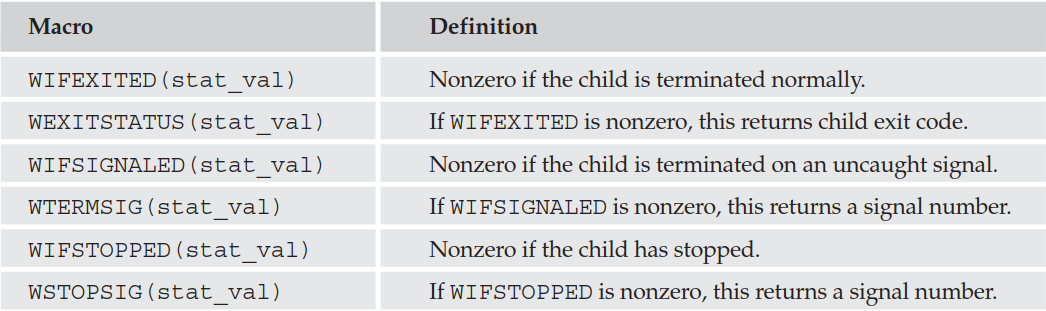
\includegraphics[width=8cm]{img/macroswait.png}
\caption{Se muestra una lista de las macros que sirven para el análisis de la variable status.}
\label{fig}
\end{figure}

\lstinputlisting[language=C]{codigos/completewait.c}

\subsubsection{Waitpid} Al igual que wait, se encarga de terminar los procesos, pero en este caso, corresponde a un proceso en especifico.

\lstinputlisting[language=C]{codigos/waitpid.c}

Recibe el pid del proceso, una variable para asignarle el estado y las flags como WNOHANG que hace que la función retorne 0 en caso de que no termine o se detenga el proceso. waitpid devolverá -1 en caso de error y establecerá errno. Esto puede ocurrir si no hay procesos hijo (errno establecido a ECHILD), si la llamada es interrumpida por una señal (EINTR), o si el argumento de opción es inválido (EINVAL).

\subsection{Pipes}

Un pipe es un canal de comunicación entre dos procesos. Se comporta como una cola (FIFO)
en donde lo que se escribe por un extremo se lee por el otro. Fue el primer mecanismo que
tuvo Unix para comunicar procesos.

Los pipes en consola son implementados con el simbolo |. Este envía el stdout al proceso de la derecha.

Un ejemplo de uso es el siguiente:

\lstinputlisting[language=C]{codigos/pipexample.txt}

En este código se implementa awk que corresponde a un lenguaje de programación de patrones y acciones diseñado para el procesamiento y análisis de texto en sistemas Unix. Al usar `\{print\}' execex.c está imprimiendo cada linea en la consola, pero al aplicar un pipe redirige la salida estandar al comando less que recibe estas lineas y las muestra en pantalla de forma interactiva.

Para trabajar con pipes en C es importante recordar lo que era los file descriptors. Estos son valores enteros mayores que cero utilizados para realizar operaciones a los archivos.

Tal como en una consola de Unix, se realizará la comunicación entre procesos mediante pipes respetando la naturaleza FIFO de este.

Se utilizarán los descriptores para lectura y escritura según correspoda. Se define entonces:

\lstinputlisting[language=C]{codigos/pipe1.c}

Donde file\_descriptor[0] será utilizado para lectura y file\_descriptor[1] para escritura.

\subsection{Ejemplo}

Se implementará una función que realice lo mismo: awk `\{print\}' codigo.c | less.

Para esto se utilizarán dos fork con exec que ejecuten los comandos a petición para posteriormente conectarlos con pipe mediante lectura y escritura definida por los descriptores.

\lstinputlisting[language=C]{codigos/pipexample2.c}

\subsubsection{\textbf{Propuesto 1}} Implementa pipes para que un proceso envíe mensajes y otro lo reciba.

\subsubsection{\textbf{Propuesto 2}} Escribe un programa en C que cuente el número de palabras en un archivo de texto. Divide la tarea entre el proceso padre y el proceso hijo. El proceso padre deberá leer el archivo y enviar las palabras al proceso hijo a través de un pipe. El proceso hijo deberá contar las palabras y enviar el resultado al proceso padre.

\subsubsection{\textbf{Propuesto 3}} Escribe un programa en C que ordene una lista de números utilizando el comando sort a través de un pipe y exec. El programa principal deberá crear un proceso hijo que ejecute sort utilizando execlp y comunicarse con el proceso hijo a través de un pipe para enviar la lista de números.

 \section{Señales}
 
Una señal es un evento generado por los sistemas UNIX y Linux en respuesta a alguna condición, tras cuya recepción un proceso puede a su vez realizar alguna acción. Usamos el término "raise" para indicar la generación de una señal, y el término "catch" para indicar la recepción de una señal. Esta señal permite controlar la ejecución de los procesos, tanto para el sistema operativo como para el usuario.

Los siguientes correspondien a posibilidades de proceso de una señal:
\begin{itemize}
\item	Terminar el proceso.
\item	Ignorar la señal.
\item	Detener el proceso.
\item	Reanudar el proceso.
\end{itemize}

Atrapar la señal mediante una función del programa

Existen una variedad de señales que se activan según una condición especifica (ver Fig. 7)
\begin{figure}[h!]
\centering
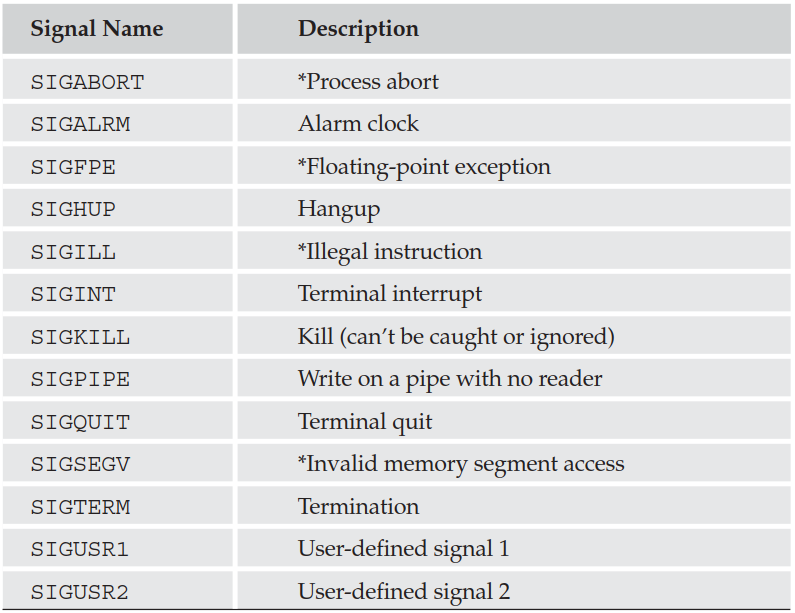
\includegraphics[width=8cm]{img/signal.png}
\caption{Se muestra una variedad de señales, el más interesante corresponde a SIGINT conocido como ctrl + C.}
\label{fig}
\end{figure}

\subsection{Signal Handling}

\subsubsection{Signal}

\lstinputlisting[language=C]{codigos/signals.c}

Esta corresponde a una declaración un tanto compleja, pero básicamente dice que esta función recibe dos parámetros. El primero corresponde a la señal que será tomada o ignorada y una función que es llamada en caso de que se reciba la señal correspondiente.

Se especifica si ignorar o no con:

\begin{itemize}
\item	SIG\_IGN para realizar la ignoración.
\item	SIG\_DFL para que la señal actue de forma predeterminada.
\end{itemize}

Podemos detectar la señal entrante implementado la función signal de la siguiente manera:

\lstinputlisting[language=C]{codigos/signal2.c}

En el momento que se presione ctrl+C se activará y imprimirá en pantalla el stdout de la función ouch.

\subsubsection{kill}

Un proceso puede enviar una señal a otro proceso, incluido él mismo, llamando a kill. La llamada fallará si el programa no tiene permiso para enviar la señal, a menudo porque el proceso de destino es propiedad de otro usuario. Este es el programa equivalente al comando del shell del mismo nombre.

\lstinputlisting[language=C]{codigos/killsig.c}

kill fallará, devolverá -1, y pondrá errno si la señal dada no es válida (errno puesto a EINVAL), si no tiene permiso (EPERM), o si el proceso especificado no existe (ESRCH).

\subsubsection{alarm}

Las señales nos proporcionan una útil función de despertador. La llamada a la función de alarma puede ser utilizada por un proceso para
programar una señal SIGALRM en algún momento en el futuro.

La llamada de alarma programa la entrega de una señal SIGALRM en segundos. De hecho, la alarma se emitirá poco después, debido a los retrasos en el procesamiento y a las incertidumbres en la programación.

\lstinputlisting[language=C]{codigos/alarm.c}

\subsubsection{Ejemplo}

\lstinputlisting[language=C]{codigos/alarm2.c}

\subsubsection{sigaction}

\lstinputlisting[language=C]{codigos/sigaction.c}

La estructura sigaction, es utilizada para definir las acciones que se llevarán a cabo al recibir la señal especificada por \textbf{sig}. Se define en signal.h y tiene al menos los siguientes atributos:

\lstinputlisting[language=C]{codigos/sigaction2.c}

La siguiente es una ejemplificación de cómo utilizar sigaction:

\lstinputlisting[language=C]{codigos/sigaction3.c}

\subsubsection{\textbf{Propuesto 1}} Implemente el código de Signal Handling de más atrás con sigaction utilizando la estructura.

\subsubsection{\textbf{Propuesto 2}} Desarrolle un programa que utilice sigaction para manejar la señal SIGTERM. Cuando el programa recibe la señal SIGTERM, deberá imprimir un mensaje y luego finalizar. En caso de no recordar que hace SIGTERM ver figura 7.

\subsubsection{\textbf{Propuesto 3}} Escribe un programa que entre en un bucle infinito y maneje las señales SIGINT y SIGTERM. Cuando se reciba SIGINT, el programa debe imprimir un mensaje indicando que se recibió SIGINT. Cuando se reciba SIGTERM, el programa debe imprimir un mensaje indicando que se recibió SIGTERM y luego finalizar de manera controlada.


\section{Bibliografía}

[1] Neil Matthew, Richard Stones. Beginning Linux Programming.
 
\end{document}
